% !TEX root = acsfubAuthorGuidelines-short.tex

% ---------------------------------------------------------------------------

% This document is with some adjustments based on

% Author guideline and sample document for EG publication using LaTeX2e input
% D.Fellner, v1.14, Nov. 29, 2017

\documentclass{egpubl}
\usepackage{eg}


\ShortPresentation % Short Conference Presentation
\electronicVersion % can be used both for the printed and electronic version

% !! *please* don't change anything above
% !! unless you REALLY know what you are doing
% ------------------------------------------------------------------------

% for including postscript figures
% mind: package option 'draft' will replace PS figure by a file name within a frame
\ifpdf \usepackage[pdftex]{graphicx} \pdfcompresslevel=9
\else \usepackage[dvips]{graphicx} \fi

\PrintedOrElectronic

% prepare for electronic version of your document
\usepackage{t1enc,dfadobe}

\usepackage{egweblnk}
\usepackage{cite}

% Define paper dimensions explicitly to avoid hyperref errors
\setlength{\paperheight}{297mm}
\setlength{\paperwidth}{210mm}

% For backwards compatibility to old LaTeX type font selection.
% Uncomment if your document adheres to LaTeX2e recommendations.
% \let\rm=\rmfamily    \let\sf=\sffamily    \let\tt=\ttfamily
% \let\it=\itshape     \let\sl=\slshape     \let\sc=\scshape
% \let\bf=\bfseries

% end of prologue

% FILMUNI: Add all your input files here
% or work directly in the acsfubAuthorGuidelines-body.tex
% !TEX root = acsfubAuthorGuidelines-short.tex

% ---------------------------------------------------------------------
% EG author guidelines plus sample file for EG publication using LaTeX2e input
% D.Fellner, v2.02, Jan 25, 2017


\title[ACS FUB \LaTeX\ Author Guidelines]%
      {\LaTeX\ Author Guidelines for the ACS FUB Proceedings Manuscripts}

% FILMUNI: for anonymous conference submission please enter your SUBMISSION ID
% instead of the author's name (and leave the affiliation blank) !!
% for final version: please provide your *own* ORCID in the brackets following \orcid; see https://orcid.org/ for more details.
\author[K. Wolf ]
{\parbox{\textwidth}{\centering K. Wolf$^{1}$}
\\
{\parbox{\textwidth}{\centering $^1$Film University Babelsberg KONRAD WOLF, Germany\\} 
}
}

%-------------------------------------------------------------------------
\begin{document}

\teaser{
    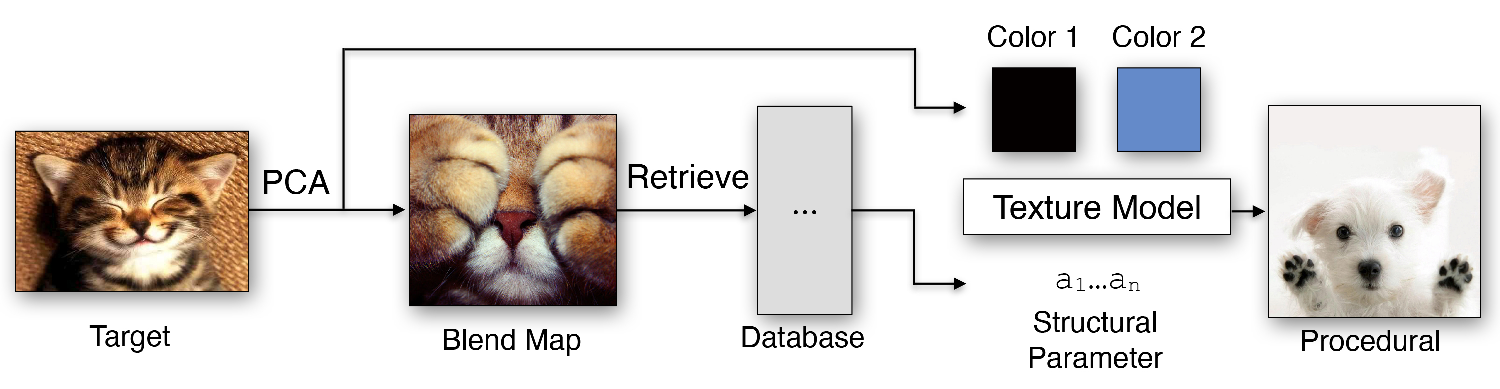
\includegraphics[width=\linewidth]{img/teaser}
    \centering
    \caption{Teaser Image. Explain the image.}
\label{fig:teaser}
}

\maketitle
%-------------------------------------------------------------------------
\begin{abstract}
 The abstract should be between 100-150 words and should be a succinct and stand alone description. An abstract is neither a summary nor an outline of the paper. For example, you can follow these four sentences \cite{johnson_1993_htg}: State the problem, Why is it a problem and why is it interesting? Your solution and achievements. What follows from your solution? 
\end{abstract}

%-------------------------------------------------------------------------
%-------------------------------------------------------------------------
\section{Introduction}

Lorem ipsum dolor sit amet, consectetur adipiscing elit. Mauris at congue arcu. Nunc sollicitudin fringilla nibh, congue interdum justo. Nunc non lacus nisi. Curabitur lacus mi, posuere vitae porttitor quis, mollis eget magna. Nam egestas lorem maximus justo tempor, non tristique ipsum dapibus. Fusce vel ultricies arcu. Morbi in quam in mauris efficitur vulputate. Quisque eu diam quis orci sagittis convallis. Pellentesque a augue sollicitudin, pellentesque nisi ut, vestibulum tortor. Nunc vitae dapibus sapien. Suspendisse a nisi ut enim cursus viverra eget in ipsum. Nullam pellentesque sollicitudin dolor, et pretium dolor egestas vel. Etiam dapibus lobortis semper. Ut vitae porttitor dui, id hendrerit nulla. Ut euismod faucibus turpis, et interdum felis sagittis id. Donec at arcu eget est elementum facilisis.

%-------------------------------------------------------------------------
%-------------------------------------------------------------------------
\section{Related Work}

Lorem ipsum dolor sit amet, consectetur adipiscing elit. Mauris at congue arcu. Nunc sollicitudin fringilla nibh, congue interdum justo. Nunc non lacus nisi. Curabitur lacus mi, posuere vitae porttitor quis, mollis eget magna. Nam egestas lorem maximus justo tempor, non tristique ipsum dapibus. Fusce vel ultricies arcu. Morbi in quam in mauris efficitur vulputate. Quisque eu diam quis orci sagittis convallis. Pellentesque a augue sollicitudin, pellentesque nisi ut, vestibulum tortor. Nunc vitae dapibus sapien. Suspendisse a nisi ut enim cursus viverra eget in ipsum. Nullam pellentesque sollicitudin dolor, et pretium dolor egestas vel. Etiam dapibus lobortis semper. Ut vitae porttitor dui, id hendrerit nulla. Ut euismod faucibus turpis, et interdum felis sagittis id. Donec at arcu eget est elementum facilisis.

%-------------------------------------------------------------------------
%-------------------------------------------------------------------------
\section{Main Content - Name and Structure the Main Content According to your Paper}

Lorem ipsum dolor sit amet, consectetur adipiscing elit. Mauris at congue arcu. Nunc sollicitudin fringilla nibh, congue interdum justo. Nunc non lacus nisi. Curabitur lacus mi, posuere vitae porttitor quis, mollis eget magna. Nam egestas lorem maximus justo tempor, non tristique ipsum dapibus. Fusce vel ultricies arcu. Morbi in quam in mauris efficitur vulputate. Quisque eu diam quis orci sagittis convallis. Pellentesque a augue sollicitudin, pellentesque nisi ut, vestibulum tortor. Nunc vitae dapibus sapien. Suspendisse a nisi ut enim cursus viverra eget in ipsum. Nullam pellentesque sollicitudin dolor, et pretium dolor egestas vel. Etiam dapibus lobortis semper. Ut vitae porttitor dui, id hendrerit nulla. Ut euismod faucibus turpis, et interdum felis sagittis id. Donec at arcu eget est elementum facilisis.

%-------------------------------------------------------------------------
\subsection{Method}

Lorem ipsum dolor sit amet, consectetur adipiscing elit. Mauris at congue arcu. Nunc sollicitudin fringilla nibh, congue interdum justo. Nunc non lacus nisi. Curabitur lacus mi, posuere vitae porttitor quis, mollis eget magna. Nam egestas lorem maximus justo tempor, non tristique ipsum dapibus. Fusce vel ultricies arcu. Morbi in quam in mauris efficitur vulputate. Quisque eu diam quis orci sagittis convallis. Pellentesque a augue sollicitudin, pellentesque nisi ut, vestibulum tortor. Nunc vitae dapibus sapien. Suspendisse a nisi ut enim cursus viverra eget in ipsum. Nullam pellentesque sollicitudin dolor, et pretium dolor egestas vel. Etiam dapibus lobortis semper. Ut vitae porttitor dui, id hendrerit nulla. Ut euismod faucibus turpis, et interdum felis sagittis id. Donec at arcu eget est elementum facilisis.

%-------------------------------------------------------------------------
\subsection{Results}

Lorem ipsum dolor sit amet, consectetur adipiscing elit. Mauris at congue arcu. Nunc sollicitudin fringilla nibh, congue interdum justo. Nunc non lacus nisi. Curabitur lacus mi, posuere vitae porttitor quis, mollis eget magna. Nam egestas lorem maximus justo tempor, non tristique ipsum dapibus. Fusce vel ultricies arcu. Morbi in quam in mauris efficitur vulputate. Quisque eu diam quis orci sagittis convallis. Pellentesque a augue sollicitudin, pellentesque nisi ut, vestibulum tortor. Nunc vitae dapibus sapien. Suspendisse a nisi ut enim cursus viverra eget in ipsum. Nullam pellentesque sollicitudin dolor, et pretium dolor egestas vel. Etiam dapibus lobortis semper. Ut vitae porttitor dui, id hendrerit nulla. Ut euismod faucibus turpis, et interdum felis sagittis id. Donec at arcu eget est elementum facilisis.

%-------------------------------------------------------------------------
\subsection{Discussion}

Lorem ipsum dolor sit amet, consectetur adipiscing elit. Mauris at congue arcu. Nunc sollicitudin fringilla nibh, congue interdum justo. Nunc non lacus nisi. Curabitur lacus mi, posuere vitae porttitor quis, mollis eget magna. Nam egestas lorem maximus justo tempor, non tristique ipsum dapibus. Fusce vel ultricies arcu. Morbi in quam in mauris efficitur vulputate. Quisque eu diam quis orci sagittis convallis. Pellentesque a augue sollicitudin, pellentesque nisi ut, vestibulum tortor. Nunc vitae dapibus sapien. Suspendisse a nisi ut enim cursus viverra eget in ipsum. Nullam pellentesque sollicitudin dolor, et pretium dolor egestas vel. Etiam dapibus lobortis semper. Ut vitae porttitor dui, id hendrerit nulla. Ut euismod faucibus turpis, et interdum felis sagittis id. Donec at arcu eget est elementum facilisis.

%-------------------------------------------------------------------------
%------------------------------------------------------------------------
\section{Formatting your paper}

%-------------------------------------------------------------------------
\subsection{Bullet Points}

The following is an example for a bullet points list. The contributions of this paper are

\begin{itemize} 
\item my greate archivement number one,
\item a second awsome insight,
\item and last but not least the third contribution.
\end{itemize}


%-------------------------------------------------------------------------
\subsection{Figures}

All graphics should be centered.

%%%
%%% Figure 1
%%%
\begin{figure}[htb]
  \centering
  % the following command controls the width of the embedded PS file
  % (relative to the width of the current column)
  
\includegraphics[width=.8\columnwidth]{img/cat_upsidedown}
  \caption{\label{fig:firstExample}
           Here is a sample figure. All figures must have sensible captions and must be referenced in the text.}
\end{figure}

If your paper includes images, it is important that they are of
sufficient resolution to be faithfully reproduced.

Instructions from the original conference template (for the ACS FUB it is not that relevant):

To determine the optimum size (width and height) of an image, measure
the image's size as it appears in your document (in millimeters), and
then multiply those two values by 12. The resulting values are the
optimum $x$ and $y$ resolution, in pixels, of the image. Image quality
will suffer if these guidelines are not followed.

Example 1: 
%
An image measures 50\,mm by 75\,mm when placed in a document. This
image should have a resolution of no less than 600 pixels by 900
pixels in order to be reproduced faithfully.

This is an examplary reference to Figure~\ref{fig:ex3}, which shows the incredible test image from the Eurogaphics conference. 


\begin{figure*}[]
    \centering
    
\includegraphics[width=.9\linewidth]{img/panda_in_tree}
    \caption{\label{fig:ex3} Two-column width figure }
\end{figure*}

%-------------------------------------------------------------------------
\subsection{Tables}

A simple table might look like the following. However there are several ways to create and layout tables - it is up to you to style a table up to your liking. This is a reference to Table \ref{tab:tableExample}.
 
\begin{table}[h!]
\centering
\begin{tabular}{|c | c c c|} 
 \hline
 Col1 & Col2 & Col2 & Col3 \\ [0.5ex] 
 \hline\hline
 1 & 6 & 87837 & 787 \\ 
 2 & 7 & 78 & 5415 \\
 3 & 545 & 778 & 7507 \\
 4 & 545 & 18744 & 7560 \\
 5 & 88 & 788 & 6344 \\ [1ex] 
 \hline
\end{tabular}
\caption{Here is a sample table. All tables must have sensible captions and must be referenced in the text.}
\label{tab:tableExample}
\end{table}



%-------------------------------------------------------------------------
\subsection{Formulas}

In \LaTeX~it is fairly easy to add mathematical symbols and formulas. See the following as example~\cite{wiki_2019_mat}:

\begin{equation} \label{eq:erl}
    a = bq + r
\end{equation}
    
which is true if $a$ and $b$ are integers with $b \neq c$.

\begin{equation}
    L' = {L}{\sqrt{1-\frac{v^2}{c^2}}}
\end{equation}


%-------------------------------------------------------------------------
\subsection{Footnotes}

Please do not use footnotes at all.


%-------------------------------------------------------------------------
\subsection{References}

References are layouted automatically. Add the needed entry to the bibtex file and use the citation command to reference the entry.

If you don't want to mention the author's name just add the citation to the end of the sentence~\cite{perlin_1985_ais}. You can also cite more than one references at the same time~\cite{gebhardt_2018_ofa, perlin_1985_ais, semmo_2015_iso}.

Sometimes you want to refer to the authors name. With this template you need to write out the names manually. For more than two authors you only use the name of the first author and abbrivate the remaining names with "et al." 

An example for more than two authors: 

Raul et al.~\cite{raut_2009_isa} thoroughly review the different approaches for segmentation algorithms. Our problem requires the segmentation of color images, summarized by Cheng et al.~\cite{cheng_2001_cis}.

An example for two authors: 

Also aiming for a fragmented aesthetic appeal by transforming original image data "piecewise", Collomosse and Hall~\cite{collomosse_2003_csr} render from salient image features a cubist version of an input. Similarly, Lai and Rosin~\cite{lai_2013_are} loosely aim for a cubist appearance by segmenting an input and by simplifying the segments into constant colors, while maintaining global structures.

An example for one author: 

Artistically, we are inspired by the art of Wehrli~\cite{wehrli_2003_tau}, who manually creates image decompositions and rearrangements.

%-------------------------------------------------------------------------
%-------------------------------------------------------------------------
\section{Conclusion}

Please direct any questions to the production editor in charge of
these proceedings.


%-------------------------------------------------------------------------

%\bibliographystyle{eg-alpha}
\bibliographystyle{eg-alpha-doi}

% FILMUNI: Add your own bib file here or
%  add your references to acsfubbib.bib
\bibliography{acsfubbib}

%-------------------------------------------------------------------------


\end{document}

